\section{Sinusformade signaler}
\textbf{HAREC a.\ref{HAREC.a.1.6}\label{myHAREC.a.1.6}}
\textbf{HAREC a.\ref{HAREC.a.1.6.1}\label{myHAREC.a.1.6.1}}

\begin{figure}[ht]
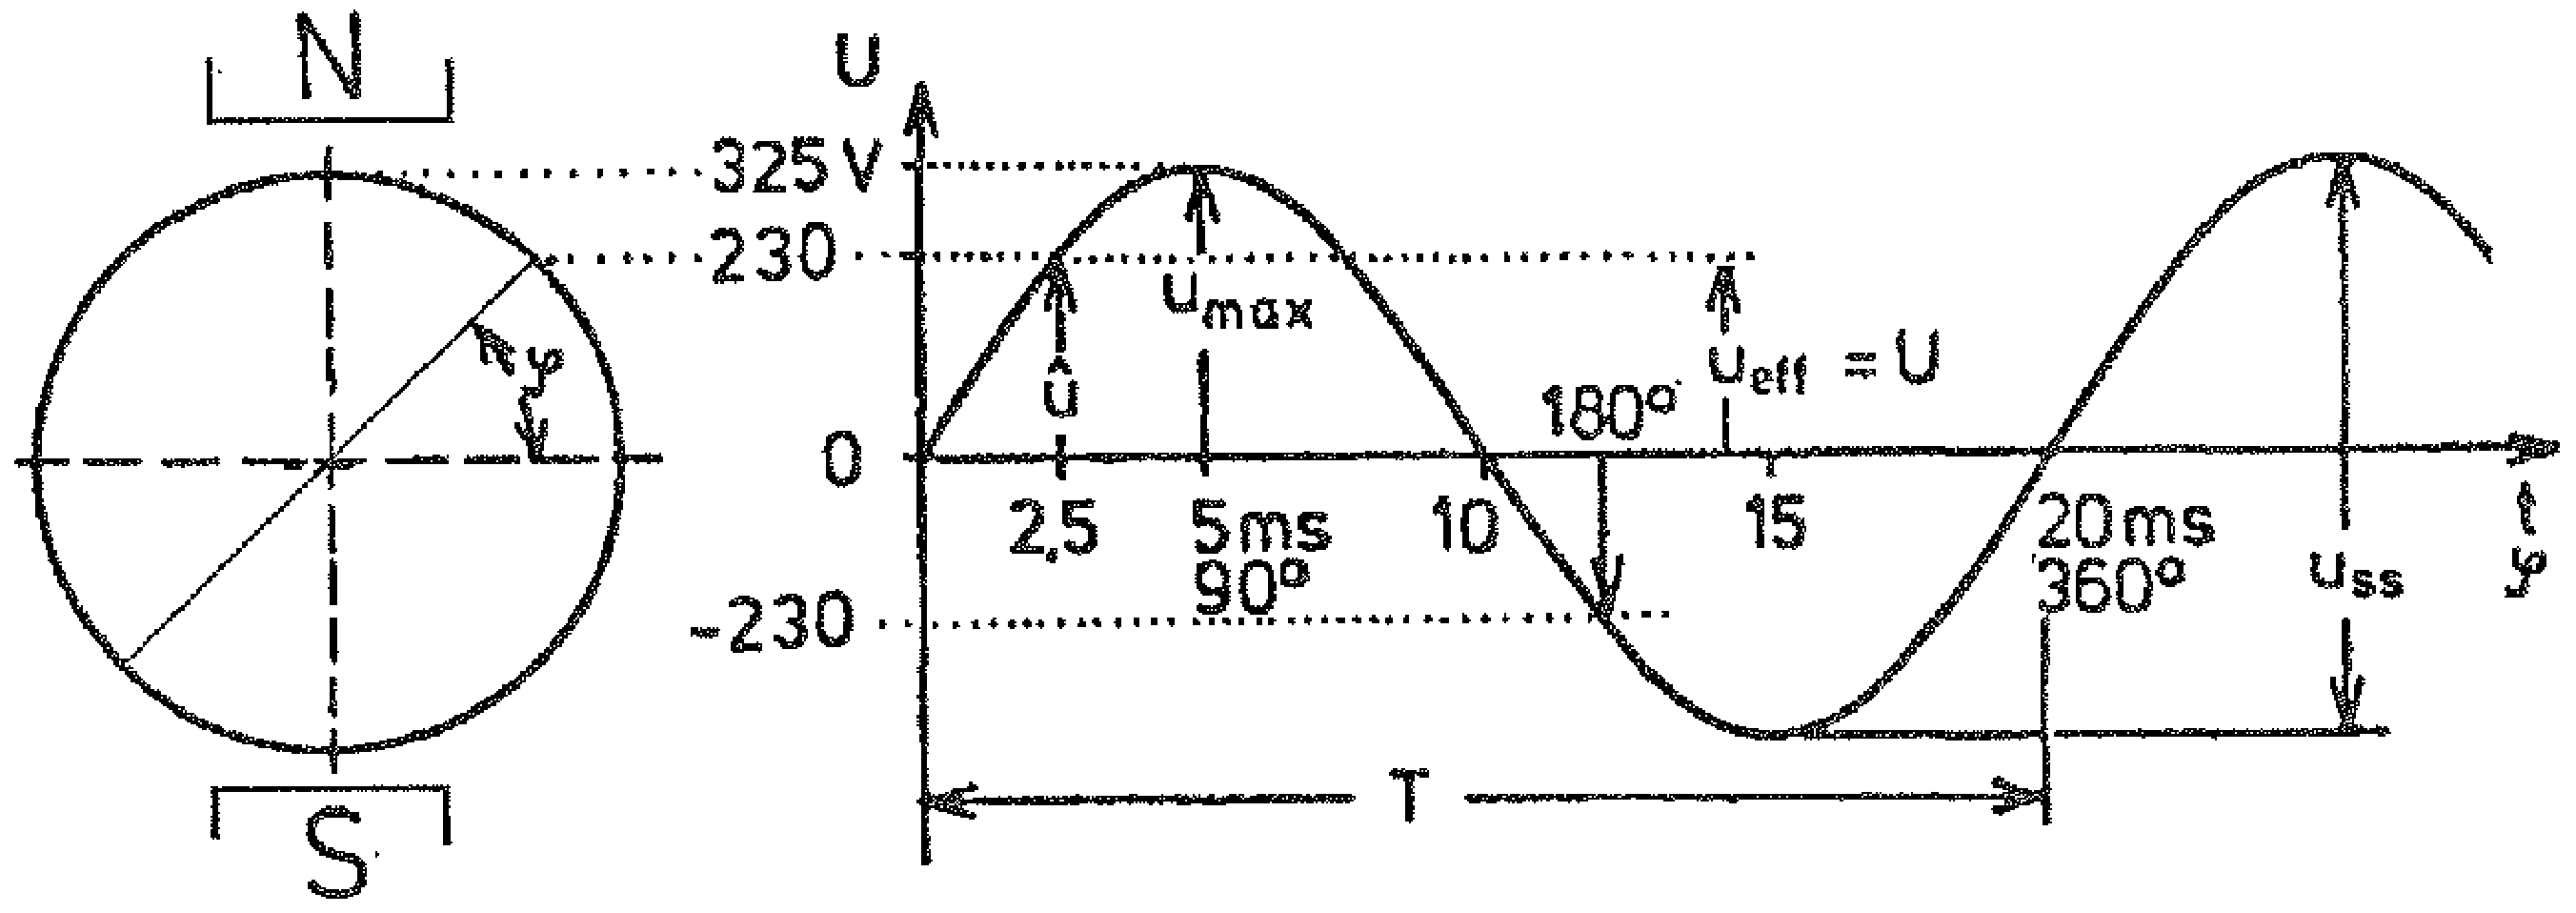
\includegraphics[width=\textwidth]{images/cropped_pdfs/bild_2_1-16.pdf}
\caption{Alstring av en sinusformad signal}
\label{fig:BildII1-16}
\end{figure}

Bild \ref{fig:BildII1-16} visar alstring av en sinusformad signal.
I detta avsnitt behandlas några grundbegrepp inom växelströmsläran.
Förloppen framställs med vektor- och linjediagram.
För närmare beskrivning används sådana begrepp som momentanvärde,
toppvärde, topp- till toppvärde, effektivvärde, fasläge, fasförskjutning och
båghastighet.

\subsection{Momentanvärde}
\textbf{HAREC a.\ref{HAREC.a.1.6.2a}\label{myHAREC.a.1.6.2a}}
\index{momentanvärde}
\index{symbol!\(u\) momentan spänning}
\index{symbol!\(i\) momentan ström}
\index{symbol!\(t\) tidpunkt}

Momentanvärdet är storheten på en spänning \(u\), en ström \(i\) etc. vid en
viss tidpunkt \(t\).
(Storheter som ändrar sig som en funktion av tiden kännetecknas ofta med gemena
bokstäver.)

Bild \ref{fig:BildII1-16} visar en sinusformad växelspänning med frekvensen
\(50\ Hz\).
Spänningen \(u\) är \(+230\ V\) vid tidpunkten 2,5~millisekunder efter en
positiv nollgenomgång.
Efter totalt \(5\, ms\) uppnås toppvärdet \(u_{max}\) dvs. \(+325\ V\).
Efter totalt \(10\, ms\) sker en negativ nollgenomgång.
Efter totalt \(12,5\, ms\) är spänningen \(-u\), dvs. \(-230\ V\) osv.

\subsection{Toppvärde eller amplitud}
\textbf{HAREC a.\ref{HAREC.a.1.6.2b}\label{myHAREC.a.1.6.2b}}
\index{toppvärde}
\index{amplitud}

Toppvärdet \(u_{max}\) är det högsta värdet över eller under noll.
På bild \ref{fig:BildII1-16} är de högsta värdena \(+325\ V\) och \(-325\ V\).

\subsection{Topp-till-toppvärde}
\index{topp-till-toppvärde}

Topp-till-toppvärde är summan av toppvärdena över och under noll.
På bild \ref{fig:BildII1-16} är detta värde \(650\ V\).

\subsection{Effektivvärde}
\textbf{HAREC a.\ref{HAREC.a.1.6.2c}, a.\ref{HAREC.a.1.6.2d}\label{myHAREC.a.1.6.2c}\label{myHAREC.a.1.6.2d}}
\index{effektivvärde}

Effektivvärdet av en växelspänning \(u\) är det värde, som medför samma
effektutveckling som en likspänning \(U\).

För ett sinusformat förlopp gäller följande samband mellan toppvärdet och
effektivvärdet (det s.k. kvadratiska medelvärdet), vilket motsvarar amplituden
vid vinklarna 45, 135, 225 och 270\degree.

\(
\begin{array}{lllll}
U=\dfrac{\hat{u}}{\sqrt{2}} & & I=\dfrac{\hat{i}}{\sqrt{2}} & & (\sqrt{2} = 1,414)
\end{array}
\)

\subsection{Fasläge}
\index{fasläge}
\index{symbol!\(\phi\) fasläge}

Fasläget \(\varphi\) är när inom en period, som ett givet momentanvärde
uppträder.
Tidpunkten för varje momentanvärde motsvarar en andel av 360\degree elektriska
grader.
Till exempel uppnås värdet volt vid 0\degree, 180\degree~och 360\degree~(= 0\degree).

\subsection{Bågmått}
\index{bågmått}
\index{radianer}
\index{båghastighet (\(\omega\))}
\index{vinkelhastighet (\(\omega\))}
\index{symbol!\(\omega\) vinkelhastighet}

I beräkningar av växelströmskretsar används ofta inte vinkelmått för fasläget
(gradtal) utan i stället begreppet bågmått.

I en s.k. enhetskrets med radien \(r = 1\) motsvaras vinkeln 360\degree av en
båge med längden \(2 \cdot \pi \cdot r= 2 \cdot \pi \cdot 1 = 2 \pi =\)
omkretsen.
Vid \(f\) perioder per sekund blir båglängden \(= 2\pi f\).
Denna storhet kallas båghastighet eller oftare vinkelhastighet och betecknas
med \(\omega\) (uttalas omega).

\(\omega= 2\pi f\) \([1/s]\)

\subsection{Period}
\textbf{HAREC a.\ref{HAREC.a.1.6.3a}\label{myHAREC.a.1.6.3a}}
\index{period}

En period har passerat, när en storhet (spänning, ström osv.) återtagit samma
tillstånd eller värde efter att ha gjort en fullständig växling, till exempel en hel
pendelrörelse eller ett helt varv vid rotation.

\subsection{Periodtid T}
\textbf{HAREC a.\ref{HAREC.a.1.6.3b}\label{myHAREC.a.1.6.3b}}
\index{periodtid (T)}
\index{symbol!\(T\) periodtid}

Periotid \(T\) är den tid som åtgår för att strömmen eller spänningen ska
genomlöpa en period. Periodtiden är det inverterade värdet av frekvensen.

Måttenheten för periodtid är sekund [s].

Periodtid

\((T) = \dfrac{1}{f}\)

\(T\ [s]  f\ [Hz]\) eller
\(T\ [ms] f\ [kHz]\) eller
\(T\ [ms] f\ [MHz]\)

Exempel:

\begin{center}
\begin{tabular}{lll}
\(T_1=\dfrac{1}{10}\) s & = 0,100 s & = 100 ms (f = 10 Hz)\\
\\
\(T_2=\dfrac{1}{50}\) s & = 0,020 s & = 20 ms (f = 50 Hz)\\
\\
\(T_3=\dfrac{1}{1000}\) s & = 0,001 s & = 1 ms (f = 1 kHz)\\
\\
\(T_4=\dfrac{1}{1000000}\) s & = 0,000001 s & = 1 \(\mu\)s (f = 1 MHz)\\
\end{tabular}
\end{center}

\subsection{Frekvens}
\textbf{HAREC a.\ref{HAREC.a.1.6.4}\label{myHAREC.a.1.6.4}}
\index{frekvens}

Frekvens är antalet perioder per tidsenhet.

Följande begrepp demonstreras med hjälp av pendeln:

Period = en fullständig fram- och tillbakasvängning i ett system, till exempel
pendelns väg mellan punkterna 2-3-2-1-2-3- osv.

\begin{figure}[ht]
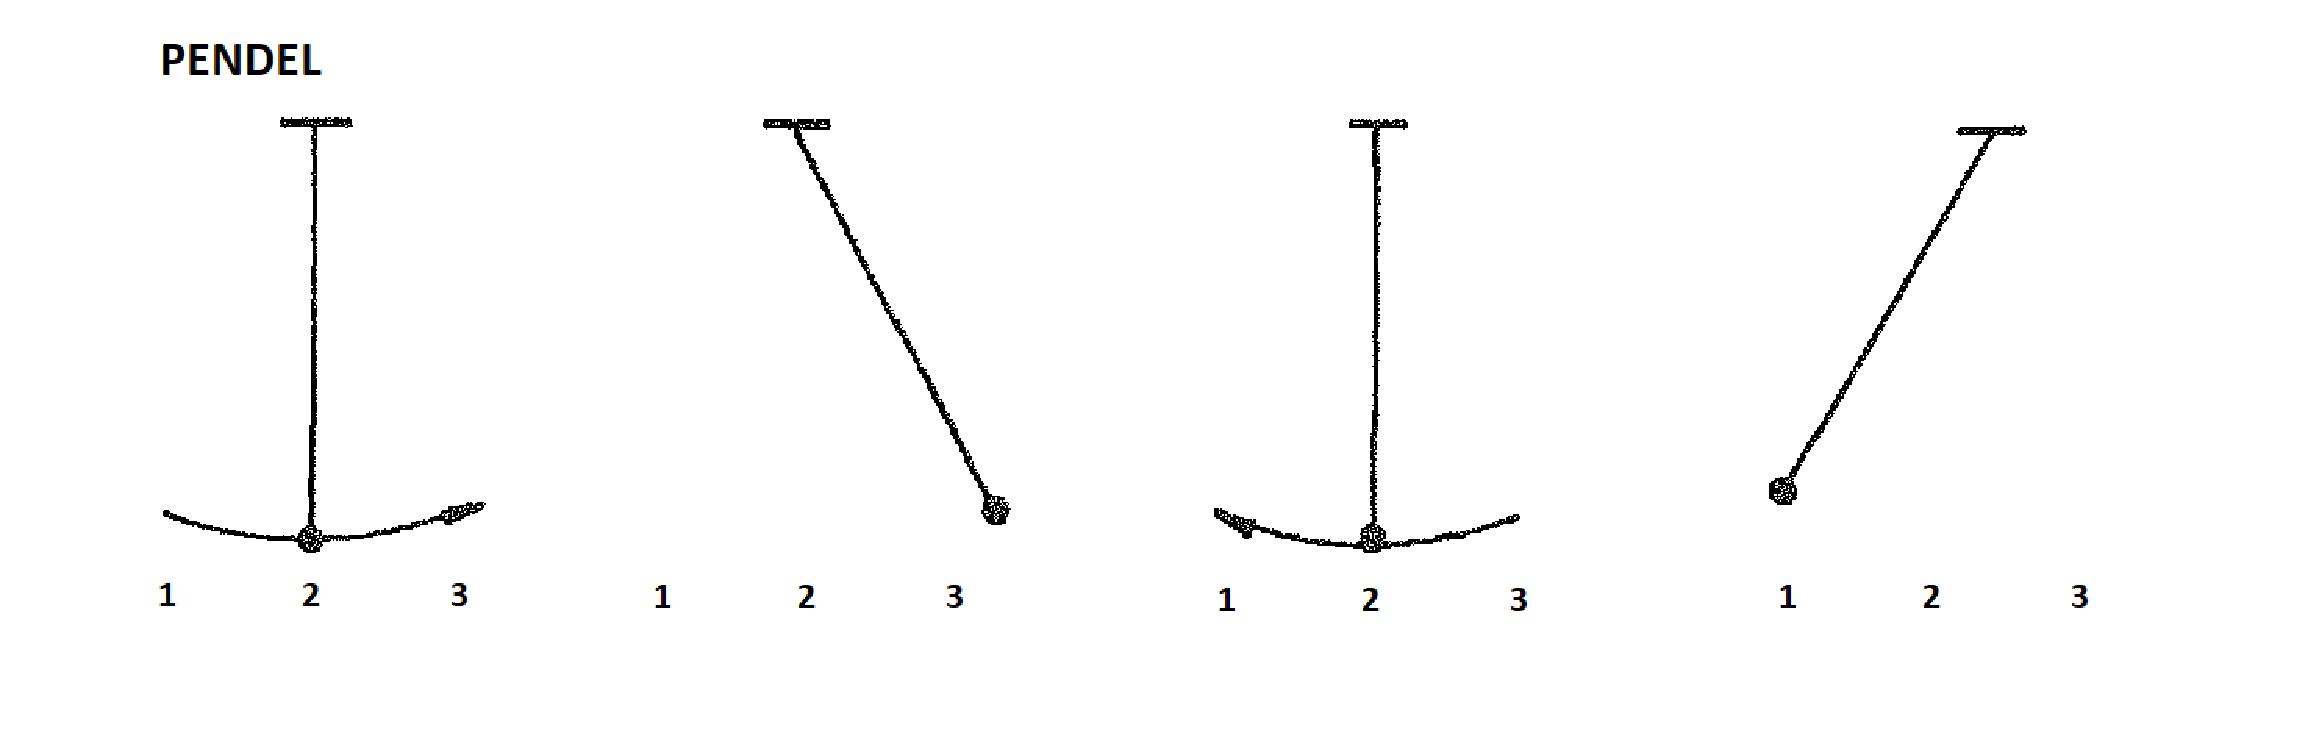
\includegraphics[width=\textwidth]{images/cropped_pdfs/bild_2_1-33.pdf}
\caption{Pendelrörelse som illustration av frekvens}
\label{fig:BildII1-33}
\end{figure}

Bild \ref{fig:BildII1-33} visar pendelrörelse som illustration av frekvens.

Periodtid \(T\) = tidsåtgången för en fullständig svängning.

Amplitud \(A\) = den största avvikelsen från viloläget.

Frekvens \(f\) = antal svängningar/tidsenhet.

Sambandet mellan frekvensen \(f\) och periodtiden \(T\) är

\(f=\dfrac{1}{T}\) till exempel

\(5 [H z] = \dfrac{1}{5}\ [sekunder]\)

\subsection{Enheten hertz}
\textbf{HAREC a.\ref{HAREC.a.1.6.5}\label{myHAREC.a.1.6.5}}
\index{hertz}
\index{enheter!hertz (Hz)}
\index{symbol!\(f\) frekvens}

Måttenheten för frekvens är hertz [Hz].
I formler betecknas frekvensen med \(f\).

\begin{center}
\begin{tabular}{ll}
1~Hz      & = 1 period per sekund (p/s) \\
10~Hz     & = 10 perioder per sekund \\
50~Hz     & = 50 perioder per sekund \\
1~000~Hz  & = \(10^3\)~Hz = 1~kHz (kilohertz) \\
1~000~kHz & = \(10^6\)~Hz = 1~MHz (megahertz) \\
1~000~MHz & = \(10^9\)~Hz = 1~GHz (gigahertz) \\
\end{tabular}
\end{center}

Nätfrekvensen för elkraft är i Europa 50~Hz.

Andra nätfrekvenser förekommer, till exempel 60~Hz i USA och Japan.

Frekvensområdet vid överföring av kvalitativt tal och musik, lågfrekvens LF, är
mellan ca 16~Hz och 16~kHz.

Frekvensområdet för talöverföring, till exempel över telefonlinjer eller
kommunikationsradio, är ca 300 till 3000~Hz.

Frekvensområdet för radioöverföring, högfrekvens HF, är i huvudsak mellan
50~kHz, s.k. långvåg, och 100-tals GHz, s.k. mikrovåg.

\subsection{Fasförskjutning}
\textbf{HAREC a.\ref{HAREC.a.1.6.6}\label{myHAREC.a.1.6.6}}
\index{fasförskjutning}

\begin{figure}[ht]
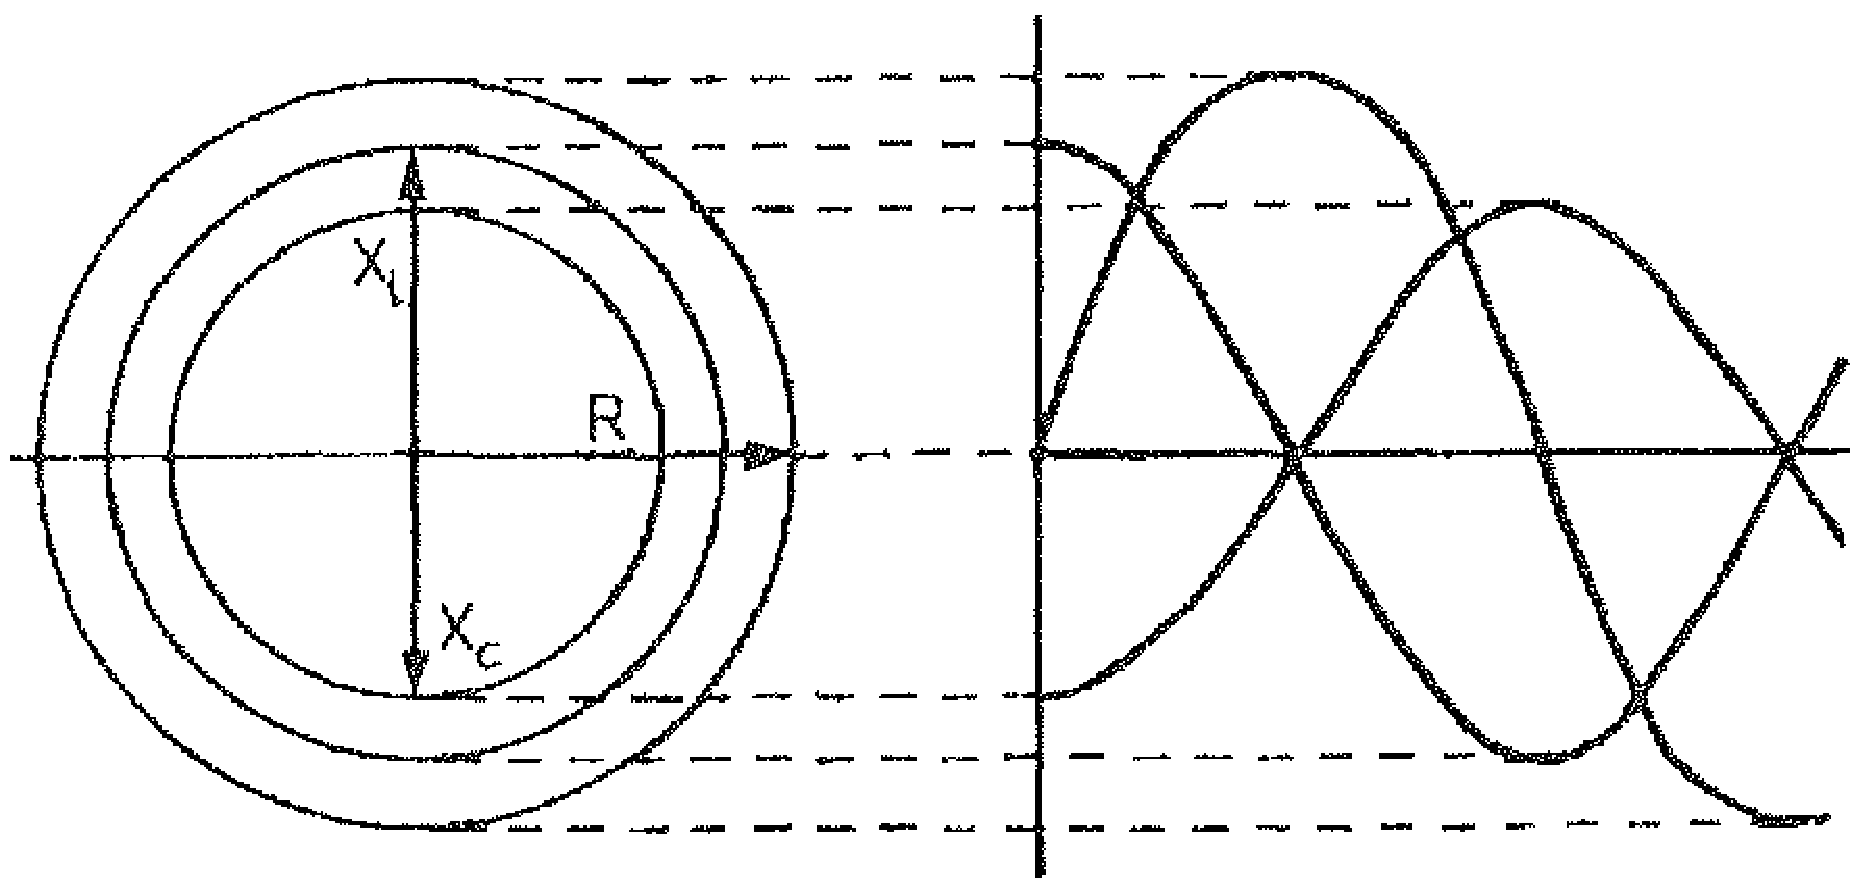
\includegraphics[width=\textwidth]{images/cropped_pdfs/bild_2_1-17.pdf}
\caption{Vektorer och fasförskjutning}
\label{fig:BildII1-17}
\end{figure}

Bild \ref{fig:BildII1-17} visar vektorer och fasförskjutning.
Med fasförskjutning menas tidsskillnaden mellan förlopp, till exempel spänningar
och/eller strömmar.
Fasförskjutningen mellan vektorerna kallas även fasvinkel och uttrycks som ett
gradtal mellan 0 och 360\degree.

\subsection{Vektorer}
\index{vektorer}

En spänning, ström, kraft osv. kan beskrivas som en vektor med en storhet och
riktning.
På bilden \ref{fig:BildII1-17} har vektorerna \(X_L\), \(R\) och \(X_C\) en
inbördes fasförskjutning av 90\degree.
De motsvarar spänningsfallen i en krets med en induktor, en resistor och en
kondensator kopplade i serie, där den gemensamma strömmen är en sinus.

Antag att vektorerna roterar i ett oförändrat inbördes läge och med en
vinkelhastighet av \(\omega= 2\pi f\).
Systemet roterar då \(360\degree = 2\pi\ radianer = 1\ varv/period\).

Vid varje tidpunkt har vektorsystemet uppnått en viss vridningsvinkel.
Momentanvärdet på vektorernas spänningar avsätts till höger i bilden.
Avståndet mellan en vektorspets och noll-linjen är vektorns momentana värde,
som kan vara positivt eller negativt.
